
%% bare_conf.tex
%% V1.4b
%% 2015/08/26
%% by Michael Shell
%% See:
%% http://www.michaelshell.org/
%% for current contact information.
%%
%% This is a skeleton file demonstrating the use of IEEEtran.cls
%% (requires IEEEtran.cls version 1.8b or later) with an IEEE
%% conference paper.
%%
%% Support sites:
%% http://www.michaelshell.org/tex/ieeetran/
%% http://www.ctan.org/pkg/ieeetran
%% and
%% http://www.ieee.org/

%%*************************************************************************
%% Legal Notice:
%% This code is offered as-is without any warranty either expressed or
%% implied; without even the implied warranty of MERCHANTABILITY or
%% FITNESS FOR A PARTICULAR PURPOSE! 
%% User assumes all risk.
%% In no event shall the IEEE or any contributor to this code be liable for
%% any damages or losses, including, but not limited to, incidental,
%% consequential, or any other damages, resulting from the use or misuse
%% of any information contained here.
%%
%% All comments are the opinions of their respective authors and are not
%% necessarily endorsed by the IEEE.
%%
%% This work is distributed under the LaTeX Project Public License (LPPL)
%% ( http://www.latex-project.org/ ) version 1.3, and may be freely used,
%% distributed and modified. A copy of the LPPL, version 1.3, is included
%% in the base LaTeX documentation of all distributions of LaTeX released
%% 2003/12/01 or later.
%% Retain all contribution notices and credits.
%% ** Modified files should be clearly indicated as such, including  **
%% ** renaming them and changing author support contact information. **
%%*************************************************************************


% *** Authors should verify (and, if needed, correct) their LaTeX system  ***
% *** with the testflow diagnostic prior to trusting their LaTeX platform ***
% *** with production work. The IEEE's font choices and paper sizes can   ***
% *** trigger bugs that do not appear when using other class files.       ***                          ***
% The testflow support page is at:
% http://www.michaelshell.org/tex/testflow/



\documentclass[conference]{IEEEtran}
% Some Computer Society conferences also require the compsoc mode option,
% but others use the standard conference format.
%
% If IEEEtran.cls has not been installed into the LaTeX system files,
% manually specify the path to it like:
% \documentclass[conference]{../sty/IEEEtran}
\usepackage{graphicx}
\usepackage{float}
\usepackage{textcomp}
\usepackage[english,brazil]{babel}

\usepackage[utf8]{inputenc}
% Some very useful LaTeX packages include:
% (uncomment the ones you want to load)


% *** MISC UTILITY PACKAGES ***
%
%\usepackage{ifpdf}
% Heiko Oberdiek's ifpdf.sty is very useful if you need conditional
% compilation based on whether the output is pdf or dvi.
% usage:
% \ifpdf
%   % pdf code
% \else
%   % dvi code
% \fi
% The latest version of ifpdf.sty can be obtained from:
% http://www.ctan.org/pkg/ifpdf
% Also, note that IEEEtran.cls V1.7 and later provides a builtin
% \ifCLASSINFOpdf conditional that works the same way.
% When switching from latex to pdflatex and vice-versa, the compiler may
% have to be run twice to clear warning/error messages.






% *** CITATION PACKAGES ***
%
%\usepackage{cite}
% cite.sty was written by Donald Arseneau
% V1.6 and later of IEEEtran pre-defines the format of the cite.sty package
% \cite{} output to follow that of the IEEE. Loading the cite package will
% result in citation numbers being automatically sorted and properly
% "compressed/ranged". e.g., [1], [9], [2], [7], [5], [6] without using
% cite.sty will become [1], [2], [5]--[7], [9] using cite.sty. cite.sty's
% \cite will automatically add leading space, if needed. Use cite.sty's
% noadjust option (cite.sty V3.8 and later) if you want to turn this off
% such as if a citation ever needs to be enclosed in parenthesis.
% cite.sty is already installed on most LaTeX systems. Be sure and use
% version 5.0 (2009-03-20) and later if using hyperref.sty.
% The latest version can be obtained at:
% http://www.ctan.org/pkg/cite
% The documentation is contained in the cite.sty file itself.






% *** GRAPHICS RELATED PACKAGES ***
%
\ifCLASSINFOpdf
% \usepackage[pdftex]{graphicx}
% declare the path(s) where your graphic files are
% \graphicspath{{../pdf/}{../jpeg/}}
% and their extensions so you won't have to specify these with
% every instance of \includegraphics
% \DeclareGraphicsExtensions{.pdf,.jpeg,.png}
\else
% or other class option (dvipsone, dvipdf, if not using dvips). graphicx
% will default to the driver specified in the system graphics.cfg if no
% driver is specified.
% \usepackage[dvips]{graphicx}
% declare the path(s) where your graphic files are
% \graphicspath{{../eps/}}
% and their extensions so you won't have to specify these with
% every instance of \includegraphics
% \DeclareGraphicsExtensions{.eps}
\fi
% graphicx was written by David Carlisle and Sebastian Rahtz. It is
% required if you want graphics, photos, etc. graphicx.sty is already
% installed on most LaTeX systems. The latest version and documentation
% can be obtained at: 
% http://www.ctan.org/pkg/graphicx
% Another good source of documentation is "Using Imported Graphics in
% LaTeX2e" by Keith Reckdahl which can be found at:
% http://www.ctan.org/pkg/epslatex
%
% latex, and pdflatex in dvi mode, support graphics in encapsulated
% postscript (.eps) format. pdflatex in pdf mode supports graphics
% in .pdf, .jpeg, .png and .mps (metapost) formats. Users should ensure
% that all non-photo figures use a vector format (.eps, .pdf, .mps) and
% not a bitmapped formats (.jpeg, .png). The IEEE frowns on bitmapped formats
% which can result in "jaggedy"/blurry rendering of lines and letters as
% well as large increases in file sizes.
%
% You can find documentation about the pdfTeX application at:
% http://www.tug.org/applications/pdftex





% *** MATH PACKAGES ***
%
%\usepackage{amsmath}
% A popular package from the American Mathematical Society that provides
% many useful and powerful commands for dealing with mathematics.
%
% Note that the amsmath package sets \interdisplaylinepenalty to 10000
% thus preventing page breaks from occurring within multiline equations. Use:
%\interdisplaylinepenalty=2500
% after loading amsmath to restore such page breaks as IEEEtran.cls normally
% does. amsmath.sty is already installed on most LaTeX systems. The latest
% version and documentation can be obtained at:
% http://www.ctan.org/pkg/amsmath





% *** SPECIALIZED LIST PACKAGES ***
%
%\usepackage{algorithmic}
% algorithmic.sty was written by Peter Williams and Rogerio Brito.
% This package provides an algorithmic environment fo describing algorithms.
% You can use the algorithmic environment in-text or within a figure
% environment to provide for a floating algorithm. Do NOT use the algorithm
% floating environment provided by algorithm.sty (by the same authors) or
% algorithm2e.sty (by Christophe Fiorio) as the IEEE does not use dedicated
% algorithm float types and packages that provide these will not provide
% correct IEEE style captions. The latest version and documentation of
% algorithmic.sty can be obtained at:
% http://www.ctan.org/pkg/algorithms
% Also of interest may be the (relatively newer and more customizable)
% algorithmicx.sty package by Szasz Janos:
% http://www.ctan.org/pkg/algorithmicx




% *** ALIGNMENT PACKAGES ***
%
%\usepackage{array}
% Frank Mittelbach's and David Carlisle's array.sty patches and improves
% the standard LaTeX2e array and tabular environments to provide better
% appearance and additional user controls. As the default LaTeX2e table
% generation code is lacking to the point of almost being broken with
% respect to the quality of the end results, all users are strongly
% advised to use an enhanced (at the very least that provided by array.sty)
% set of table tools. array.sty is already installed on most systems. The
% latest version and documentation can be obtained at:
% http://www.ctan.org/pkg/array


% IEEEtran contains the IEEEeqnarray family of commands that can be used to
% generate multiline equations as well as matrices, tables, etc., of high
% quality.




% *** SUBFIGURE PACKAGES ***
%\ifCLASSOPTIONcompsoc
%  \usepackage[caption=false,font=normalsize,labelfont=sf,textfont=sf]{subfig}
%\else
%  \usepackage[caption=false,font=footnotesize]{subfig}
%\fi
% subfig.sty, written by Steven Douglas Cochran, is the modern replacement
% for subfigure.sty, the latter of which is no longer maintained and is
% incompatible with some LaTeX packages including fixltx2e. However,
% subfig.sty requires and automatically loads Axel Sommerfeldt's caption.sty
% which will override IEEEtran.cls' handling of captions and this will result
% in non-IEEE style figure/table captions. To prevent this problem, be sure
% and invoke subfig.sty's "caption=false" package option (available since
% subfig.sty version 1.3, 2005/06/28) as this is will preserve IEEEtran.cls
% handling of captions.
% Note that the Computer Society format requires a larger sans serif font
% than the serif footnote size font used in traditional IEEE formatting
% and thus the need to invoke different subfig.sty package options depending
% on whether compsoc mode has been enabled.
%
% The latest version and documentation of subfig.sty can be obtained at:
% http://www.ctan.org/pkg/subfig




% *** FLOAT PACKAGES ***
%
%\usepackage{fixltx2e}
% fixltx2e, the successor to the earlier fix2col.sty, was written by
% Frank Mittelbach and David Carlisle. This package corrects a few problems
% in the LaTeX2e kernel, the most notable of which is that in current
% LaTeX2e releases, the ordering of single and double column floats is not
% guaranteed to be preserved. Thus, an unpatched LaTeX2e can allow a
% single column figure to be placed prior to an earlier double column
% figure.
% Be aware that LaTeX2e kernels dated 2015 and later have fixltx2e.sty's
% corrections already built into the system in which case a warning will
% be issued if an attempt is made to load fixltx2e.sty as it is no longer
% needed.
% The latest version and documentation can be found at:
% http://www.ctan.org/pkg/fixltx2e


%\usepackage{stfloats}
% stfloats.sty was written by Sigitas Tolusis. This package gives LaTeX2e
% the ability to do double column floats at the bottom of the page as well
% as the top. (e.g., "\begin{figure*}[!b]" is not normally possible in
% LaTeX2e). It also provides a command:
%\fnbelowfloat
% to enable the placement of footnotes below bottom floats (the standard
% LaTeX2e kernel puts them above bottom floats). This is an invasive package
% which rewrites many portions of the LaTeX2e float routines. It may not work
% with other packages that modify the LaTeX2e float routines. The latest
% version and documentation can be obtained at:
% http://www.ctan.org/pkg/stfloats
% Do not use the stfloats baselinefloat ability as the IEEE does not allow
% \baselineskip to stretch. Authors submitting work to the IEEE should note
% that the IEEE rarely uses double column equations and that authors should try
% to avoid such use. Do not be tempted to use the cuted.sty or midfloat.sty
% packages (also by Sigitas Tolusis) as the IEEE does not format its papers in
% such ways.
% Do not attempt to use stfloats with fixltx2e as they are incompatible.
% Instead, use Morten Hogholm'a dblfloatfix which combines the features
% of both fixltx2e and stfloats:
%
% \usepackage{dblfloatfix}
% The latest version can be found at:
% http://www.ctan.org/pkg/dblfloatfix




% *** PDF, URL AND HYPERLINK PACKAGES ***
%
%\usepackage{url}
% url.sty was written by Donald Arseneau. It provides better support for
% handling and breaking URLs. url.sty is already installed on most LaTeX
% systems. The latest version and documentation can be obtained at:
% http://www.ctan.org/pkg/url
% Basically, \url{my_url_here}.




% *** Do not adjust lengths that control margins, column widths, etc. ***
% *** Do not use packages that alter fonts (such as pslatex).         ***
% There should be no need to do such things with IEEEtran.cls V1.6 and later.
% (Unless specifically asked to do so by the journal or conference you plan
% to submit to, of course. )


% correct bad hyphenation here
\hyphenation{op-tical net-works semi-conduc-tor}

\begin{document}
	\title{Riscos no Desenvolvimento de Software}
	
	\author{\IEEEauthorblockN{Higor de Oliveira Chaves}
		\IEEEauthorblockA{Universidade Federal\\ do Mato Grosso do Sul\\
			Coxim, MS 79400--000\\
			Telefone: (67) 99896-4797\\
			Email: higor.chaves@aluno.ufms.br}
		\and
		\IEEEauthorblockN{Rafael Gon\c{c}alves de Oliveira Viana}
		\IEEEauthorblockA{Universidade Federal\\ do Mato Grosso do Sul\\
			Coxim, MS 79400--000\\
			Telefone: (67) 99950-7979\\
			Email: rafael.viana@aluno.ufms.br} 
		\and
		\IEEEauthorblockN{Ramon da Silva V. dos Santos}
		\IEEEauthorblockA{Universidade Federal\\do Mato Grosso do Sul\\
			Coxim, MS 79400--000\\
			Telefone: (67) 98114--5649\\
			Email: ramon.santos@aluno.ufms.br}
		}
	
	\maketitle
	
	\begin{abstract}
		
		Existe atualmente um grande volume de dados sendo transmitidos pelos mais diversos dispositivos disseminados na sociedade mundial. A tendência do mundo moderno, é que esses dados tornem-se um recurso natural, que como qualquer outro, necessita ser refinado para que possa ser bem utilizado. Para que essa grande massa de dados se torne informação útil e relevante porém, algumas técnicas precisam ser aplicadas, técnicas estas que necessitam de um grande poder computacional. Neste artigo, será demonstrado a diferença de perfomance entre CPU e GPU em algoritmos que necessitam de muito processamento. Para tal objetivo foram utilizadas as bibliotecas TensorFlow e cuDDN juntamente com a plataforma CUDA. 
		
		\begin{IEEEkeywords} Data Science, GPU, CUDA, TensorFlow. \end{IEEEkeywords}
	\end{abstract}
	
	
	
	\IEEEpeerreviewmaketitle
	
	
	\section{Introdução}
	Com a chegada do conceito de \textit{BigData} e com a atual tendência de sensoriar tudo e todos, a rede mundial de computadores tem se tornado uma grande e complexa mina de ouro. Esta mina porém, não contém apenas dados bons e relevantes, para chegar a essas características, deve-se passar por um processo de mineração, onde as informações inúteis são descartadas e as relevantes conservadas. À descoberta de conhecimento, extração e preservação apenas do que é útil, dá-se o nome de \textit{Data Science}.
	
	Assim como na mineração de recursos naturais, a mineração de dados necessita de ferramentas e técnicas robustas para que seja possível realizar um maior e melhor processamento. Estas técnicas no entanto, demandam muito poder de máquina e por conta disso são extremamente custosas. Além disso, a mineração é apenas uma das etapas de um grande e complexo sistema de análise e refinamento de dados.
	
	Para obter informações valiosas, como por exemplo a probabilidade de um produto ser vendido em determinada região, ou a predição de ações na bolsa de valores, os dados são tratados utilizando diversas técnicas de \textit{Data Science} - agrupamento, filtro, classificação, entre outras, que assim como a mineração, demandam muito processamento.
	
	Afim de amenizar a lentidão causada por algoritmos que necessitam de muito recurso computacional, será apresentado neste artigo como a GPU pode se tornar um grande auxiliar no processamento massivo de dados, paralelizando as tarefas e tornando assim o processo como um todo mais veloz.
	
	
	\section{Fundamenta\c{c}\~ao Te\'orica}
	
	
	\subsection{GPGPU}
	
	Al\'em de trabalhos de artistas e desenvolvedores de jogos, trabalhos inovadores com a tecnologia come\c{c}aram a sugir, assim ouve o nascimento do movimento da GPU de Prop\'osito Geral  - \textit{GPGPU}.
	
	\subsection{KDD}
	\textit{Knowledge Discovery in Database} ou Descoberta de Conhecimento em Bando de Dados, tem uma função muito importante na produção de conhecimento neste artigo, pois a extração de conhecimento que é usada por esta técnica, não é simplesmente coletar os dados, e sim um conjunto de etapas, para chegar em um resultado refinado.
	
	\subsection{CUDA}
	CUDA \'e uma plataforma de computa\c{c}\~ao paralela inventada pela NVIDIA. Ela \'e capaz de aumentar significativamente a performance computacional ao utilizar e aproveitar a pot\^encia da unidade de processamento gr\'afico GPU.
	
	
	
	O CUDA Toolkit conta com um compilador, bibliotecas de matem\'aticas e ferramentas para depura\c{c}\~ao e otimiza\c{c}\~ao da performance de seus aplicativos, para ficar melhor ele   \'e distribu\'ido gratuitamente, al\'em de sua documenta\c{c}\~ao e manuten\c{c}\~ao fornecidos pela NVIDIA.
	
	\subsection{cuDDN}
	\'E uma biblioteca para o NVIDIA CUDA, para rede neurais profunda que fornece implementa\c{c}\~oes altamente sintonizadas para rotinas padr\~ao, como convolu\c{c}\~ao para tr\'as (propaga\c{c}\~ao), agrupamento, normaliza\c{c}\~ao e camadas de ativa\c{c}\~ao.
	Diversos softwares de redes profundas dependem do cuDDN (Caffe2, MatLab, Microsofot Cognitive Toolkit, TensorFlow, Theano, PyTorch) para acelerac\c{c}\~ao GPU de alto desempenho, permitindo se concentrar no treinamento de rede neurais e no desenvolvimento de aplica\c{c}\~oes em vez de gastar tempo no ajuste de desempenho de GPU de baixo n\'ivel.
	
	\subsection{TensorFlow}
	O TensorFlow desenvolvida pela Google é uma biblioteca  de técnicas em Inteligência Artificial inovadora e conta com uma comunidade ativa. O TensorFlow pode ser usado por indivíduos em busca de pesquisas ou mesmo grandes empresas que precisam implementar estratégias.
	

	
	\section{An\'alise de T\'ecnicas}
	
	Existem c\'alculos computacionais como os utilizados na engenharia, m\'idia digital e aplica\c{c}\~oes cient\'ificas que exigem grande poder de processamento, onde a CPU n\~ao consegue um bom desempenho. 
	
	As GPUs atuam como um co-processador e podem acelerar as aplica\c{c}\~oes devido ao seu poder de processamento massivamente paralelo em rela\c{c}\~ao ao design dos v\'arios n\'ucleos das CPUs.
	
	Nesta sess\~ao iremos apresentar a técnica de multiplicação de Matrizes, onde a mesma e utilzada por diversas outras técnicas \cite{IEEEhowto:3}.
	
	
	\subsection{Multiplica\c{c}\~ao de Matrizes}
	
	Esse \'e um exemplo trivial da computa\c{c}\~ao pelo seu grande gasto computacional, um exemplo pr\'atico s\'eria algumas redes neurais convolucional de classifica\c{c}\~ao de imagem, que utiliza o produto das matrizes para cria\c{c}\~ao de filtros.
	
	Um exemplo pr\'atico pode ser observado na Tabela \ref{an:mult}, onde foram apresentados tr\^es testes de 150\texttwosuperior, 1500\texttwosuperior , 15000\texttwosuperior, todos com valores internos rand\^omicos, a GPU somente foi superior no teste quando o n\'ivel de complexidade relativamente grande.
	
	\begin{table}[H]
		\centering
		\caption{Demonstração}
		\label{an:mult}
		\begin{tabular}{clcc}
			\hline
			\multicolumn{1}{l}{\textbf{Tamanho da Matriz}} &  & \multicolumn{1}{l}{\textbf{Tempo na CPU ms}} & \multicolumn{1}{l}{\textbf{Tempo na GPU ms}} \\ \hline
			150 X 150                                      &  & 0:00.137                                     & 0:00.668                                     \\
			1500 X 1500                                    &  & 0:00.318                                     & 0:00.661                                     \\
			15000 X 15000                                  &  & 2:36.198                                     & 0:10.329                                     
		                                \\ \hline
		\end{tabular}
	\end{table}
	
	\subsubsection{Camada Convolucional}
	A convolução é uma operação matemática utilizada processamento único para filtrar sinais, identificar padrões em sinais. Em uma camada convolucional, todos os neurônios aplicam operação de convolução às entradas, portanto, são chamados de neurônios convolucionais. O parâmetro mais importante em um neurônio convolucional é o tamanho do filtro, digamos que temos uma camada com tamanho de filtro 5 * 5 * 3. Além disso, suponha que a entrada que é alimentada ao neurônio convolucional é uma imagem de entrada de tamanho de 32 * 32 com 3 canais, como na Figura abaixo \cite{IEEEhowto:4}. 
	
	\begin{figure}[H]
		\centering
		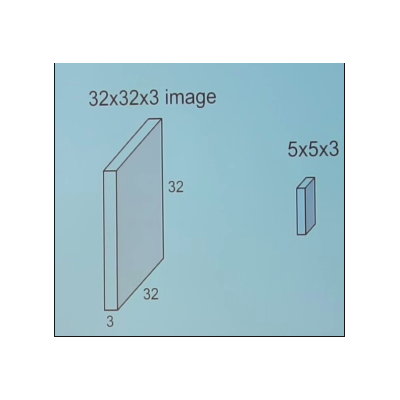
\includegraphics[scale=0.2]{imagen/1.png}
		
		\caption{Criação de um filtro com uma parcela da imagen.}
		\label{figRotulo}
	\end{figure}
	Após algumas técnicas dividadas em camadas de neurônios (como a camada de agrupamento e a totalmente conectada), o algoritmo converge reconhecendo os padrões através dos pixels multiplicados.
	O resultado desse processo e a Figura 2, que contém um vetor de padrões reconhecidos \cite{IEEEhowto:3}.

	 \begin{figure}[H]
		\centering
		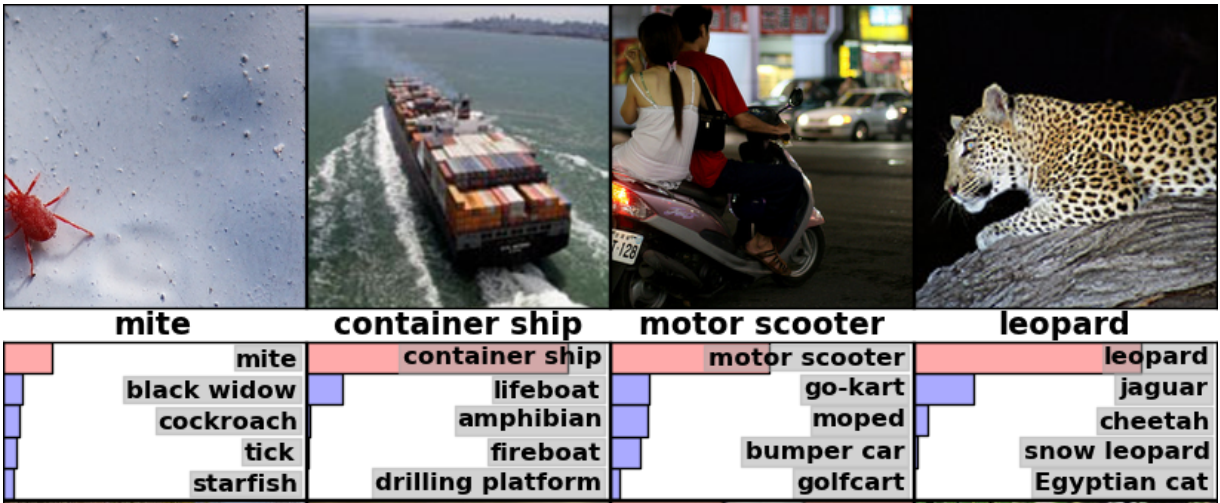
\includegraphics[scale=0.15]{imagen/AlexClassification.png}
		
		\caption{Foto com vetor de padrões reconhecidos}
		\label{figRotulo}
	\end{figure}
	\section*{Conclus\~ao}
	O processamento paralelo em GPU tem grande difiren\c{c}a quando os dados computados s\~ao de grande complexidade, o que torna essa tarefa muito custosa para a CPU, tornando assim a GPU uma otima opção ao aproveitar sua paralelização  nesses c\'alculos, por\'em para c\'alculos computacionais de baixa complexidade a CPU, se mostrou superior na velocidade do processamento.
	
	
	\begin{thebibliography}{1}
		
		
		\bibitem{IEEEhowto:4}
		Campos V., Sastre F., Maurici Y., Jordi Torres and Xavier G. \emph{Scaling a Convolutional Neural Network for
			classification of Adjective Noun Pairs with
			TensorFlow on GPU Clusters}\hskip 1em plus
		0.5em minus 0.1em\relax Barcelona
		Supercomputing Center - Centro Nacional de Supercomputación (BSC), 2017.
		
		
		
		\bibitem{IEEEhowto:2}
	Monard, Maria Carolina and Baranauskas, Jos{\'e} Augusto \emph{Conceitos sobre aprendizado de m{\'a}quina}\hskip 1em plus
		0.5em minus 0.1em\relax Sistemas Inteligentes-Fundamentos e Aplica{\c{c}}{\~o}es, 2003.
		
		\bibitem{IEEEhowto:7}
	M. Abadi, P. Barham, J. Chen, Z. Chen, A. Davis, J. Dean,
	M. Devin, S. Ghemawat, G. Irving, M. Isard, M. Kudlur,
	...\emph{TensorFlow: A System for Large-Scale
		Machine Learning}\hskip 1em plus
	0.5em minus 0.1em\relax 
	12th USENIX Symposium on Operating Systems Design
	and Implementation (OSDI ’16), 2016.
			\bibitem{IEEEhowto:3}
		Marcelo H. and Santos S., R. Leal, Jos{\'e} Alberto and KIM, HaeYong\emph{	Classifica{\c{c}}{\~a}o de imagens de sensoriamento remoto pela aprendizagem por {\'a}rvore de decis{\~a}o: uma avalia{\c{c}}{\~a}o de desempenhos}\hskip 1em plus
		0.5em minus 0.1em\relax Simp{\'o}sio Brasileiro de Sensoriamento Remoto, 2005.
		
		
		
		\bibitem{IEEEhowto:1}
		R. Sujith, \emph{ProjectionNet: Learning Efficient On-Device Deep			Networks Using Neural Projections }\hskip 1em plus
		0.5em minus 0.1em\relax Google Research, 2017.
			\bibitem{IEEEhowto:5}
		K. Wongsuphasawat, D. Smilkov, J. Wexler, J. Wilson,
		D. Mané, D. Fritz, D. Krishnan, Fernanda B. Viégas, and Martin W.\emph{Visualizing Dataflow Graphs of
			Deep Learning Models in TensorFlow}\hskip 1em plus
		0.5em minus 0.1em\relax 17th IEEE/ACM International Symposium on Cluster, Cloud and Grid Computing, 2017.
		
		
			\bibitem{IEEEhowto:6}
		Young J., J. Kim , Jong-Kook K. , A. Mohaisen, and Woojoo L.\emph{Performance of Deep Learning Computation with
			TensorFlow Software Library in GPU-Capable
			Multi-Core Computing Platforms}\hskip 1em plus
		0.5em minus 0.1em\relax School of Computer Science and Engineering, Chung-Ang University, Seoul, Republic of Korea, 2017.
		
		
		
		
	
	\end{thebibliography}
	
	
\end{document}


